\chapter{Genetic Programming}\label{ch:gp}

\section{Introduction}

\bfit{Genetic Programming (GP)} is a specialized domain within evolutionary computation where the individuals of the population are not fixed-length strings representing parameters, but executable computer programs. Popularized by John Koza in the late 1980s, GP aims to stochastically evolve populations of programs to find one that performs a user-defined task satisfactorily.

While the high-level evolutionary cycle of GP is analogous to that of a Genetic Algorithm (involving initialization, fitness evaluation, selection, and variation through crossover and mutation) the core of GP's uniqueness lies in its representation. Instead of evolving solutions \textit{to} a problem, GP \textit{evolves the problem-solving logic itself}.

This shift in representation from data structures to programs opens up a vast application space, from symbolic regression and controller design to automatic programming and machine learning model discovery.

\begin{figure}[H]
    \centering
    \includegraphics[width=0.7\textwidth]{assets/gp-cycle.png} % Corresponds to slide 5
    \caption{\centering The general evolutionary cycle in Genetic Programming, which closely mirrors the cycle of a standard GA but operates on programs instead of fixed-length genotypes.}
    \label{fig:gp_cycle}
\end{figure}

\vspace{-1em}

The fundamental challenge of GP's power, is finding a program representation that can be effectively manipulated by genetic operators to create syntactically valid and semantically useful offspring.

\section{Program Representation}

Representing programs as linear strings, similar to GAs, is problematic. Applying standard crossover to raw source code strings often results in syntactically invalid offspring, as the operator has no awareness of the underlying program structure. This is because the crossover point is likely to break syntax, resulting in non-compilable or nonsensical offspring. To overcome this problem, GP typically represents programs as \bfit{syntax trees} (or expression trees).

\subsection{Tree-Based Representation}


In the tree-based representation, each program is structured as a rooted tree: \textbf{internal nodes} correspond to functions or operators, while the \textbf{leaf nodes} are terminals, which can be variables or constants. This tree-based structure offers several key advantages for genetic programming:

\begin{minipage}{0.55\textwidth}

\vspace{0.5em}
\begin{itemize}
    \item \textbf{Modularity:} Any subtree forms a valid, self-contained sub-program or expression, enabling flexible manipulation and reuse of code fragments.
    \item \textbf{Closure and Validity:} Genetic operators can operate on entire subtrees, ensuring that offspring remain syntactically valid and executable.
    \item \textbf{Interpretability:} The hierarchical structure mirrors the way mathematical and logical expressions are naturally composed, making evolved programs easier to visualize and understand.
    \item \textbf{Fitness Evaluation:} The output of a program can be computed by recursively evaluating the tree from the leaves up to the root, allowing for efficient and systematic fitness assessment.
\end{itemize}
\end{minipage}
\hspace{1em}
\begin{minipage}{0.40\textwidth}
\begin{figure}[H]
    \centering
    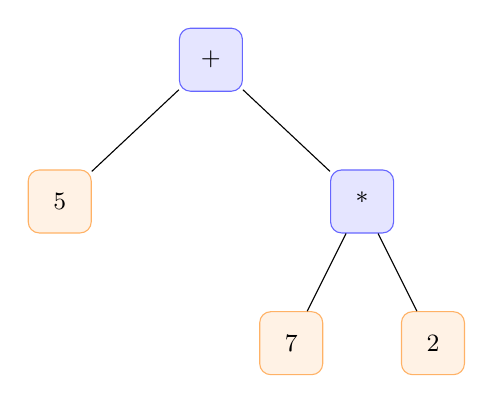
\begin{tikzpicture}[scale=1.2, level distance=1.5cm,
      every node/.style={font=\small,draw,rounded corners,minimum size=8mm,inner sep=2pt},
      level 1/.style={sibling distance=3.2cm},
      level 2/.style={sibling distance=1.5cm}]
      % Root
      \node[fill=blue!10,draw=blue!60] (plus) {\plaintt{+}}
        child {node[fill=orange!10,draw=orange!60] {\plaintt{5}}}
        child {node[fill=blue!10,draw=blue!60] {\plaintt{*}}
          child {node[fill=orange!10,draw=orange!60] {\plaintt{7}}}
          child {node[fill=orange!10,draw=orange!60] {\plaintt{2}}}
        };
    \end{tikzpicture}
    \caption{ \textbf{The expression $5 + (7 \times 2)$ as a syntax tree.} Internal nodes represent functions or operators (\plaintt{+}, \plaintt{*}), while leaf nodes are terminals (5, 7, 2).
    }
    \label{fig:gp_tree_example}
\end{figure}
\end{minipage}

\subsubsection{Terminals and Functions}

A Genetic Programming (GP) system is built from two fundamental sets of building blocks, which together define the "language" in which solutions can be expressed:

\begin{itemize}
    \item \bfit{Terminal Set} ($\mathcal{T}$): contains all possible leaf nodes of the tree, elements that do not take any arguments. Terminals are the basic inputs and constants that the evolved programs can use. Typical examples include:
    \begin{itemize}
        \item \textbf{Input Variables:} represent the problem-specific inputs, such as $x_0, x_1, \ldots, x_n$.
        \item \textbf{Constants:} fixed values such as numbers, or logical values (\texttt{true}, \texttt{false}).
    \end{itemize}

    \item \bfit{Function Set} ($\mathcal{F}$): This set contains all possible internal nodes, elements that take one or more arguments (their \textit{arity}), corresponding to their child nodes in the tree. The function set determines the kinds of computations and logic the GP system can evolve. Examples include:
    \begin{itemize}
        \item \textbf{Arithmetic Operators:} \texttt{+}, \texttt{-}, \texttt{*}, \texttt{/} (often with protected division to avoid errors).
        \item \textbf{Trigonometric Functions:} \texttt{sin}, \texttt{cos}, \texttt{tan}, etc.
        \item \textbf{Boolean Operators:} \texttt{AND}, \texttt{OR}, \texttt{NOT}, \texttt{XOR}, etc., for logical or rule-based problems.
        \item \textbf{Conditional Constructs:} \texttt{IF-ELSE}, \texttt{IF-GREATER}, etc., enabling programs to make decisions.
        \item \textbf{Other Domain-Specific Functions:} functions as \texttt{abs}, \texttt{log}, \texttt{exp}, or user-defined primitives.
    \end{itemize}
\end{itemize}
The combination of $\mathcal{T}$ and $\mathcal{F}$ forms the \bfit{primitive set}, which specifies the fundamental components available to the GP system for constructing solutions.

\begin{tipsblock}[Primitive Set]
    Choosing the primitive set is important: it should be \bfit{expressive enough} to represent solutions, but \bfit{not so large or complex} that it makes the search inefficient or the evolved programs unnecessarily complicated.
\end{tipsblock}

\subsubsection{Properties of the Primitive Set}
The choice of primitives is critical and must satisfy two important properties for the GP system to function correctly.


\begin{itemize}
    \item \textbf{Closure}
    
    The \bfit{closure} property requires that any function in $\mathcal{F}$ must be able to accept any value returned by another function or any terminal from $\mathcal{T}$. This ensures that any tree constructed from the primitives is valid. It has two main aspects:
    \begin{itemize}
        \item \textbf{Type Consistency:} All functions, operators, and terminals must operate on and return the same data type (or be part of a strongly-typed GP system that can handle multiple types). For example, if all functions expect numbers, a terminal returning \texttt{true} would violate closure.
        \item \textbf{Evaluation Safety:} Functions prone to runtime errors must be "protected." For example, \texttt{safe\_div(a, b)} returns 1 if $b=0$, avoiding division-by-zero during evaluation.
    \end{itemize}

    \vspace{0.5em}

    \item \textbf{Sufficiency}
    
    The \bfit{sufficiency} property requires that the primitive set must be capable of representing a solution to the problem. For instance, if the target function is an exponential, but the primitive set only contains polynomials and variables, it may be impossible to find an exact solution. While perfect sufficiency is often not knowable in advance, the set should be chosen to be rich enough to allow for good approximations.
\end{itemize}


\section{Initialisation, Crossover and Mutation}

\subsection{Population Initialisation}
Unlike the straightforward random initialisation of binary strings in a GA, generating a population of valid, random program trees in GP requires a more structured approach. The aim is to produce a diverse set of trees with varying sizes and shapes. The most widely used method for this is \bfit{Ramped Half-and-Half}.

\subsubsection{Ramped Half-and-Half}

This method combines two fundamental tree-generation strategies:

\begin{itemize}
    \item \textbf{The Grow Method}: nodes are randomly selected from the entire primitive set ($\mathcal{F} \cup \mathcal{T}$) as the tree is built, up to a specified maximum depth. Once a branch reaches this maximum depth, only terminals from $\mathcal{T}$ can be chosen. This approach tends to produce \bfit{asymmetric trees} of various shapes and sizes, since a branch may terminate before reaching the maximum depth if a terminal is selected at an internal node.

    \item \textbf{The Full Method}: nodes are chosen exclusively from the function set $\mathcal{F}$ until the maximum depth is reached. At this depth, all leaf nodes are filled with terminals from $\mathcal{T}$. This results in "bushy" \bfit{full trees} where all terminals are located at the same depth.
\end{itemize}

To ensure diversity in the initial population, the \textbf{Ramped Half-and-Half} method works as follows:
\begin{enumerate}
    \item A range of maximum depths is defined (e.g., from 2 to 6).
    \item The population is divided into groups, each assigned a maximum depth from this range.
    \item For each depth group, half of the individuals are generated using the \textit{grow} method and the other half using the \textit{full} method.
\end{enumerate}
This approach guarantees that the initial population contains a broad variety of program structures and sizes, which is essential for effective evolutionary search.

\subsubsection{Ephemeral Constants}
When a problem requires numeric constants, they can be pre-defined in the terminal set (e.g., $\mathcal{T} = \{x, y, 1, \pi\}$). However, a more flexible approach is the use of \bfit{ephemeral constants}. An ephemeral constant is a special terminal that, when selected, generates a random constant within a predefined range (e.g., a random float in $[-1, 1]$). Each time this terminal appears in a tree, it holds a different, randomly generated value.

\vspace{-1em}

\begin{figure}[H]
    \centering
    \begin{minipage}{0.65\textwidth}
        \centering
        \includegraphics[width=\textwidth]{assets/gp-ephemeral.png}
        \captionof{figure}{\centering The \textit{Ephemeral} terminal generates a random constant in $[0, 3]$. Each instance holds a different random value.}
        \label{fig:gp_ephemeral}
    \end{minipage}
\end{figure}

\vspace{-1.5em}

\subsection{Crossover}
The standard crossover operator in GP is \textbf{subtree crossover}. It operates as follows:
\begin{enumerate}[noitemsep]
    \item Two parent trees are selected from the population.
    \item A random node (the crossover point) is chosen in each parent tree.
    \item Swap the selected subtrees between parents to create one or two offspring.
\end{enumerate}

\vspace{-1em}

\begin{figure}[H]
    \centering
    \begin{minipage}{0.65\textwidth}
        \centering
        \includegraphics[width=\textwidth]{assets/gp-crossover.png}
        \captionof{figure}{\centering Subtree Crossover.}
        \label{fig:gp_crossover}
    \end{minipage}
\end{figure}

\vspace{-1em}

This operator is simple yet powerful, as it combines potentially useful, self-contained building blocks (subtrees) from different parents. A common constraint is to enforce a maximum depth on offspring to prevent them from growing excessively large after crossover.

\begin{observationblock}[Non-Homologous Crossover]
    Unlike one-point or uniform crossover in GAs, which align genes by position (\bfit{homologous}), subtree crossover is \bfit{non-homologous}. The exchanged subtrees can come from different positions and depths and have different sizes and shapes. This allows for a more flexible and dynamic exchange of genetic material.
\end{observationblock}


\subsection{Mutation}
In GP, mutation involves making a small, random change to a single parent tree. There are several common mutation operators, each with a different effect:

\begin{itemize}
    \item \bfit{Subtree Mutation:} A random crossover point is selected in the tree, and the entire subtree rooted at that point is replaced by a new, randomly generated tree (often using the \texttt{grow} method). This is a major mutation, capable of drastically changing the program's behavior.
    
    \vspace{-0.5em}
    
    \begin{figure}[H]
        \centering
        \includegraphics[width=0.5\textwidth]{assets/gp-subtree-mutation.png}
    \end{figure}

    \vspace{-1em}
        
    \item \bfit{Point Mutation:} A random node in the tree is replaced by another primitive from the set. To maintain validity, a function can only be replaced by a function of the same arity, and a terminal can only be replaced by another terminal. This is a much smaller, more targeted change than subtree mutation.
    
    \vspace{-1em}

    \begin{figure}[H]
        \centering
        \includegraphics[width=0.5\textwidth]{assets/gp-point-mutation.png}
    \end{figure}

    \vspace{-1em}

    \item \bfit{Hoist Mutation:} A random subtree is selected from within the tree, and this subtree becomes the new, complete tree. This is a size-reducing operator, as it replaces the entire tree with one of its smaller parts.
    
    \vspace{-1em}

    \begin{figure}[H]
        \centering
        \includegraphics[width=0.5\textwidth]{assets/gp-hoist-mutation.png}
    \end{figure}

    \vspace{-1em}

    \item \bfit{Shrink Mutation:} A randomly selected subtree is replaced by a single, randomly chosen terminal. This is another effective operator for reducing program size.
    
    \vspace{-1em}

    \begin{figure}[H]
        \centering
        \includegraphics[width=0.5\textwidth]{assets/gp-shrink-mutation.png}
    \end{figure}

    \vspace{-1em}

    \item \bfit{Permutation Mutation:} The arguments of a selected function are permuted. For a binary operator, this would mean swapping its two child subtrees. This is most effective for non-commutative functions.
    
    \vspace{-0.5em}

    \begin{figure}[H]
        \centering
        \includegraphics[width=0.5\textwidth]{assets/gp-permutation-mutation.png}
    \end{figure}

\end{itemize}

\subsection{The Genetic Operators in Action}

Let's provides a visual overview of the main steps in a typical Genetic Programming (GP) evolutionary cycle. The \cref{fig:gp_example} shows how an initial population of program trees is evaluated for fitness, followed by the selection of individuals based on their fitness values. The selected individuals then undergo genetic operations such as crossover, where subtrees are exchanged to create new offspring, and mutation, where random changes are introduced to maintain diversity. This process is repeated over successive generations to evolve better solutions.

\begin{figure}[H]
    \centering
    \includegraphics[width=0.75\textwidth]{assets/gp-example.png}
\end{figure}


\section{Code Re-use: Automatically Defined Functions (ADF)}

A fundamental limitation of standard Genetic Programming is that, when a useful code fragment (i.e. a subtree) is required in multiple locations within a program, the evolutionary process must independently evolve this fragment each time it is needed. To address this inefficiency and to promote modularity and code reuse, the concept of \bfit{Automatically Defined Functions (ADFs)} was introduced, drawing inspiration from \textit{subroutines} in conventional programming languages.

With ADFs, an individual is no longer a single tree but a \bfit{forest} of trees, comprising:
\begin{itemize}
    \item A primary \textbf{result-producing branch}, which serves as the main program tree.
    \item One or more \textbf{function-defining branches}, each corresponding to a distinct ADF.
\end{itemize}
Each ADF has a unique identifier (e.g., `ADF1`, `ADF2`) and a fixed arity, with arguments denoted (e.g., `ARG1`, `ARG2`). These ADFs may be invoked as functions within the main program tree or within other ADFs, thereby enabling the construction of hierarchical and nested function calls.

\vspace{-0.5em}

\begin{figure}[H]
    \centering
    \includegraphics[width=0.55\textwidth]{assets/gp-adf.png}

    \vspace{-0.5em}

    \captionof{figure}{\centering \small Illustration of Automatically Defined Functions (ADFs).}
\end{figure}

\vspace{-1.2em}

When employing ADFs, genetic operators are applied to all trees within the forest. For instance, crossover may occur between the main program trees of two parent individuals, between their respective ADF trees, or between an ADF tree and a main program tree. This co-evolutionary mechanism enables GP to autonomously discover and exploit useful, reusable submodules.

\section{Bloat and Parsimony Pressure}

\subsubsection{Bloat}

A common and challenging problem in GP is \bfit{bloat}: the tendency for programs to grow in size over generations without a corresponding improvement in fitness. This happens because larger trees can often have more neutral crossover or mutation points, giving them a slight selective advantage.

\vspace{-1em}

\begin{minipage}{0.55\textwidth}

One major symptom of bloat is the emergence of large \textbf{non-coding regions}, also known as \bfit{introns}. These are sections of code that have no effect on the final output (e.g., a subtree like \texttt{(x - x)}, which always evaluates to 0, or an \texttt{IF} statement that is never taken).

\vspace{0.5em}

Bloat is problematic because it significantly increases the computational cost of fitness evaluations, slowing down the evolutionary process.

\end{minipage}%
\begin{minipage}{0.45\textwidth}
\begin{figure}[H]
    \centering
    \includegraphics[width=0.85\textwidth]{assets/gp-bloat.png}
    \captionof{figure}{\centering \small Illustration of bloat in GP.}
    \label{fig:gp_bloat}
\end{figure}
\end{minipage}

\vspace{-2em}

\subsubsection{Controlling Bloat}
Several methods are used to combat bloat:
\begin{enumerate}
    \item \textbf{Strict Size/Depth Limits:} The most direct method is to impose a hard maximum limit on tree depth or the number of nodes. Offspring that exceed this limit after are discarded.
    
    \item \textbf{Size-Reducing Operators:} Including mutation operators like \texttt{Hoist} and \texttt{Shrink} in the evolutionary process can help counteract growth.
    
    \item \textbf{Parsimony Pressure:} This widely used technique modifies the fitness function to penalize larger trees, creating selection pressure for both correctness and simplicity. A common approach is to use a weighted combination of fitness and size:
    $$
      f_{adj}(p) = \alpha f(p) - (1-\alpha)\,\text{size}(p)
    $$
    Here, $f(p)$ is the original fitness of program $p$, $\text{size}(p)$ is its size (number of nodes), and $\alpha \in [0,1]$ is a parameter that balances the importance of fitness versus parsimony. When $\alpha$ is close to 1, fitness dominates; when it is smaller, parsimony is emphasized.
\end{enumerate}

\begin{figure}[H]
    \centering
    \includegraphics[width=0.55\textwidth]{assets/gp-parsimony.png}
\end{figure}

\begin{tipsblock}[Parsimony Pressure Tuning]
    The parameter $\alpha$ must be chosen carefully. If it is too close to 1, bloat will not be controlled. If it is too small, evolution may be stifled by penalizing necessary complexity, resulting in trivial, low-fitness solutions. Its value is often tuned empirically to balance the two objectives.
\end{tipsblock}

\section{Alternative Program Representations}

While tree-based representation is the canonical form of Genetic Programming, it is not the only one. Several alternative representations have been developed to address some of the challenges of tree-based GP or to better suit specific problem domains, such as evolving imperative programs or designing digital circuits. These methods often replace the explicit tree structure with a linear genotype that is either executed directly or used to generate a more complex phenotype.

\subsection{Linear Genetic Programming (LGP)}

\bfit{Linear Genetic Programming (LGP)} departs from the LISP-like expression trees and instead represents programs as a linear sequence of instructions, much like a program in assembly language.

\subsubsection{Representation and Execution}
In LGP, an individual is a variable-length sequence of simple instructions that operate on a set of registers. The program is executed by interpreting these instructions sequentially, and the final result is typically read from a designated output register after execution.

\begin{figure}[H]
    \centering
    \includegraphics[width=0.6\textwidth]{assets/lgp-example.png}
    \caption{\centering An example of a Linear GP individual.}
    \label{fig:lgp_example}
\end{figure}

\vspace{-1em}

\begin{observationblock}[LGP vs. Genetic Algorithms]
    At first glance, LGP's linear genotype seems very similar to that of a standard GA. However, there is a crucial distinction:
    \begin{itemize}
        \item In a GA, the genotype \textit{is} the solution.
        \item In LGP, the genotype is a \textit{program} that must be executed to produce a result. The fitness is determined by the outcome of this execution, not by the instruction sequence itself. This introduces a complex genotype-to-phenotype mapping.
    \end{itemize}
\end{observationblock}

\subsubsection{Genetic Operators in LGP}
Since the representation is linear, LGP can adapt standard GA operators.
\begin{itemize}
    \item \bfit{Crossover:} A common approach is a two-point crossover. Since individuals can have different lengths, the crossover points in each parent are chosen independently. A segment of instructions is then swapped between the two parents.
    \item \bfit{Mutation:} Mutation can take several forms, such as changing an instruction's operator (e.g., \texttt{ADD} to \texttt{SUB}), altering a register pointer, or modifying a constant value. Macro-mutations, like inserting or deleting an entire instruction, are also used to change the program's length.
\end{itemize}

\subsection{Cartesian Genetic Programming (CGP)}

\bfit{Cartesian Genetic Programming (CGP)} is a form of genetic programming introduced by Julian F. Miller. In CGP, candidate programs are represented as \textbf{directed acyclic graphs} (DAGs). This representation is particularly well-suited for tasks involving multiple inputs and outputs. Although the phenotype (the expressed program) is a graph, the underlying genotype is a linear, fixed-length string of integers, similar in spirit to the representation used in LGP.

\subsubsection{Representation and Encoding}
A CGP individual consists of a two-dimensional grid of computational nodes, typically organized into a specified number of rows and columns. Each node in the grid implements a function selected from a predefined function set.

\begin{figure}[H]
    \centering
    \includegraphics[width=0.7\textwidth]{assets/cgp-ex.png}
    \caption{\centering Genotype-to-phenotype mapping in CGP.}
    \label{fig:cgp_example}
\end{figure}

\begin{itemize}
    \item The \textbf{genotype} is a fixed-length sequence of integers. It encodes the following information:
        \begin{enumerate}
            \item For each node in the grid:
                \begin{itemize}
                    \item The function to be computed by the node (identified by an index into the function set).
                    \item The source of each input to the node, specified as the address (index) of either a program input or an output from a preceding node in the grid.
                \end{itemize}
            \item For each program output:
                \begin{itemize}
                    \item The address (index) of the node whose output is to be used as the program's final output.
                \end{itemize}
        \end{enumerate}
    \item Each node is typically encoded by a fixed group of integers (a \textit{gene}), for example: \texttt{[function\_id, input1\_addr, input2\_addr]}.
    \item The complete genotype is formed by concatenating the genes for all nodes, followed by the output node addresses.
\end{itemize}

\begin{figure}[H]
    \centering
    \includegraphics[width=0.7\textwidth]{assets/cgp-example.png}
    \caption{\centering CGP individual and its genotype.}
    \label{fig:cgp_encoding}
\end{figure}

\vspace{-1em}

\begin{tipsblock}[Non-Coding Genes in CGP]
    A key feature of CGP is that not all nodes in the grid need to be part of the final, active graph that connects inputs to outputs. Nodes whose outputs are not used by any subsequent active node are effectively non-coding genes (introns). This neutrality is believed to be beneficial for the evolutionary search, allowing genetic changes to accumulate without immediate phenotypic effect.
\end{tipsblock}

\subsubsection{Genetic Operators in CGP}
Evolution in CGP is typically driven exclusively by \textbf{mutation}. A common strategy is a (1+$\lambda$)-ES, where a parent generates $\lambda$ offspring via mutation, and the fittest individual among the parent and offspring survives. Crossover is rarely used.
\bfit{Point mutation} is the primary operator: one or more integers in the genotype are randomly changed to another valid value. This can either change a node's function or re-wire its connections.

\subsection{Grammatical Evolution (GE)} \label{sec:ge}
\bfit{Grammatical Evolution (GE)} offers a powerful bridge between the simplicity of a linear genome and the structural complexity of high-level languages. Instead of evolving program trees directly, GE evolves a sequence of integers which, guided by a formal grammar, deterministically generates a syntactically correct program. This approach separates the genotype (the integer string) from the phenotype (the final program).

\subsubsection{Backus-Naur Form (BNF) Grammar}
The core engine of GE is a context-free grammar, specified in \bfit{Backus-Naur Form (BNF)}. Invented by John Backus and Peter Naur for the ALGOL language, a BNF grammar formally defines a language as a set of production rules. A grammar is a quadruple $(\mathcal{T}, \mathcal{N}, \mathcal{P}, \mathcal{S})$:
\begin{itemize}
    \item \bfit{Terminals ($\mathcal{T}$):} The set of final (non-expandable) symbols that form the language's strings.
    \item \bfit{Non-Terminals ($\mathcal{N}$):} The set of abstract symbols that can be expanded into other symbols.
    \item \bfit{Production Rules ($\mathcal{P}$):} A set of rules mapping a non-terminal to a sequence of terminals and/or non-terminals. The pipe symbol \texttt{|} is used to denote alternative expansions.
    \item \bfit{Start Symbol ($\mathcal{S}$):} The specific non-terminal where the expansion process begins.
\end{itemize}

\begin{exampleblock}[BNF Grammar for Sum of Integers]
    Consider the following grammar from the slides:
    \begin{multicols}{2}
    \begin{itemize}
        \item $\mathcal{T} = \{+, 0, 1, 2, 3, 4, 5, 6, 7, 8, 9\}$
        \item $\mathcal{N} = \{S, C, D\}$
        \item $\mathcal{S} = S$
    \end{itemize}
    \columnbreak
    \begin{itemize}
        \item $\mathcal{P}: \ \ 
        \begin{array}{l}
            S \to S+S \mid C \\
            C \to D \mid DC \\
            D \to 0 \mid 1 \mid 2 \mid 3 \mid 4 \mid 5 \mid 6 \mid 7 \mid 8 \mid 9
        \end{array}
        $
    \end{itemize}
    \end{multicols}
    This grammar can generate strings representing the sum of any positive integers (e.g., "42+8+6"). The expansion process, or \bfit{derivation}, starts with $S$ and repeatedly applies rules to expand non-terminals until only terminals remain. For example:
    $$
        S \to S+S \to C+S \to DC+S \to \ldots \to 42+8+6
    $$
    This derivation can also be viewed as the construction of a syntax tree, where non-terminals are internal nodes and terminals are the leaves.
\end{exampleblock}

\subsubsection{The Genotype-to-Phenotype Mapping}
GE uses a linear vector of integers, called \textbf{codons}, as its genotype. This genome guides the derivation process. To generate a program (phenotype), GE performs the following steps:
\begin{enumerate}[noitemsep]
    \item Start the derivation string with the axiom $\mathcal{S}$.
    \item Read the next codon from the genome.
    \item Identify the leftmost non-terminal in the current derivation string.
    \item Count the number $N_r$ of alternative production rules available for this non-terminal.
    \item Select which rule to apply using the formula: $\text{rule\_index} = \text{codon} \pmod{N_r}$.
    \item Replace the non-terminal with the chosen expansion.
    \item Repeat from step 2 until only terminals are left in the string or a termination limit is reached.
\end{enumerate}

\vspace{-0.5em}

\begin{figure}[H]
    \centering
    \includegraphics[width=0.5\textwidth]{assets/ge.jpg}
    \caption{\centering The core mapping mechanism in GE.
    \\
    An integer codon is used to select a production rule via the modulo operator.}
    \label{fig:ge_mapping}
\end{figure}

\vspace{-1.5em}

\begin{exampleblock}[Full Derivation Walkthrough]
        Let's consider the following grammar:
        $$
        \begin{array}{lcll}
            S & \to & (S \text{ OP } S) \mid V \mid N & \quad \text{(3 choices)} \\
            OP & \to & + \mid \times \mid - \mid \div & \quad\text{(4 choices)} \\
            V & \to & x_1 \mid x_2 \mid x_3 & \quad\text{(3 choices)} \\
            N & \to & \text{-}DD \mid \text{-}D \mid D \mid DD & \quad\text{(4 choices)} \\
            D & \to & 0 \mid 1 \mid \ldots \mid 9 & \quad\text{(10 choices)}
        \end{array}
        $$
        and the genome:
        $$[3, 5, 22, 6, 9, 2, 56, 18, 24, 1]$$
    
        \vspace{0.5em}
        \begin{minipage}[t]{0.69\textwidth}
        \textbf{Mapping Process:}

        \begin{enumerate}[nosep, leftmargin=2em, labelwidth=!, labelindent=0pt]
            \item Start with axiom \texttt{S}.
            \item Read codon \textbf{3}. For \texttt{S} (3 choices), rule is $3 \pmod 3 = 0$.
            \item Read codon \textbf{5}. For \texttt{S} (3 choices), rule is $5 \pmod 3 = 2$.
            \item Read codon \textbf{22}. For \texttt{N} (4 choices), rule is $22 \pmod 4 = 2$.
            \item \dots
        \end{enumerate}

        \vspace{1em}

        The process continues, always expanding the leftmost non-terminal using the next available codon. The final phenotype is the program $(5 \times x_2)$.

        \vspace{1em}

        Note that the last three codons are not used in the derivation.
    \end{minipage}%
    \hfill
    \begin{minipage}[t]{0.28\textwidth}
        \vspace{-2em}
        \small
        $$
        \boxed{
            \begin{array}{l}
                \text{\textbf{Full Derivation Chain:}} \\[1em]
                \begin{array}{llll}
                    \underline{S} & \to \ (\underline{S} \text{ OP } S) & \ [0]\\[0.5em]
                                  & \to \ (\underline{N} \text{ OP } S) & \ [2]\\[0.5em]
                                  & \to \ (\underline{D} \text{ OP } S) & \ [2]\\[0.5em]
                                  & \to \ (5 \text{ \underline{OP} } S) & \ [6]\\[0.5em]
                                  & \to \ (5 \times \underline{S}) & \ [1]\\[0.5em]
                                  & \to \ (5 \times \underline{N}) & \ [1]\\[0.5em]
                                  & \to \ (5 \times \underline{V}) & \ [1]\\[0.5em]
                                  & \to \ (5 \times x_2)
                \end{array}
            \end{array}
        }
        $$
    \end{minipage}
    \end{exampleblock}

\subsubsection{Unique Properties and Challenges}
The indirect genotype-phenotype mapping in GE leads to several distinctive characteristics:
\begin{itemize}
    \item \bfit{Variable-Length Genomes and Wrapping:}
    
    Genomes can have different lengths. If the derivation process exhausts all codons before the program is complete, GE can "wrap around" and reuse codons from the beginning of the genome.

    
    \item \bfit{Handling Incomplete Derivations:}
    
    To prevent infinite recursions (e.g. $S \to S+S \to S+S+S \to \ldots$), a maximum number of derivation steps is enforced. If a genome fails to produce a complete program within this limit, it is deemed invalid and assigned a very low fitness score.

    \item \bfit{Degeneracy and Neutrality:}
    
    There is no one-to-one mapping between genotype and phenotype. Many different integer genomes can produce the exact same final program. This is known as degeneracy and is a source of neutral mutations (changes in the genotype that do not change the phenotype), which can be beneficial for traversing the fitness landscape.
    
    \item \bfit{Epistasis and the Ripple Effect:}
    
    The function of a gene is highly dependent on the genes that came before it, as they determine the sequence of derivation steps. A single mutation early in the genome can cause a "ripple effect," completely changing how the rest of the codons are interpreted and leading to a radically different phenotype.
\end{itemize}

\subsubsection{Genetic Operators for GE}
Since the genotype is a linear vector of integers, GE can leverage standard GA operators.
\begin{itemize}
    \item \textbf{Crossover:} One-point and two-point crossover are commonly used.
    \item \textbf{Mutation:} Randomly replaces a codon with a new integer.
\end{itemize}
More advanced, GE-specific crossover operators also exist. For example, \textbf{sensible crossover} is a one-point crossover that uses the actual effective length of each individual. Other operators include \textbf{ripple crossover}, and \textbf{homologous crossover}, which attempts to align two genomes based on their derivation history and perform crossover at points where their derivations begin to differ, aiming for a more meaningful exchange of information.

\begin{figure}[H]
    \centering
    \includegraphics[width=0.65\textwidth]{assets/ge-homologous.png}
    \caption{\centering Homologous crossover in GE.}
    \label{fig:ge_homologous}
\end{figure}

\begin{tipsblock}[PonyGE2]
Grammatical evolution is available in the \textbf{PonyGE2} library:

\begin{center}
    \url{https://github.com/PonyGE/PonyGE2}
\end{center}

\textbf{Tip:} To install PonyGE2, you must \textit{clone or download} the repository from GitHub. 

\textbf{You cannot use \plaintt{pip} or Anaconda for installation.}
\end{tipsblock}